% !TEX root = ../Dokumentation.tex
\section{Technologierecherche}
\subsection{Funktionsweise der Hardware}
Für die geplante Arbeit wird ein Raspberry Pi 3, eine 32GB SD-Karte, eine Basisplatine, Sensorplatinen mit Temperaturfühlern sowie entsprechende Verbindungskabel verwendet. Das Raspberry Pi ist ein Einplatinencomputer und eignet sich mit seinen Funktionen und Komponenten besonders gut für diese Arbeit. Über die elektrischen Anschlusspunkte, auch GPIOs genannt, werden die Messsignale des Temperatursensors abgefragt. Mittels der Basisplatine, welche an das Raspberry angeschlossen wird, können die gelieferten Daten der angeschlossenen Sensoren von einem analogen zu einem digitalen Signal umgewandelt werden.
Diese digitalen Signale können so in Temperaturwerte umgerechnet und für eine kontinuierliche Anzeige bereitgestellt werden.

\begin{figure}[H]%Position festigen
\centering
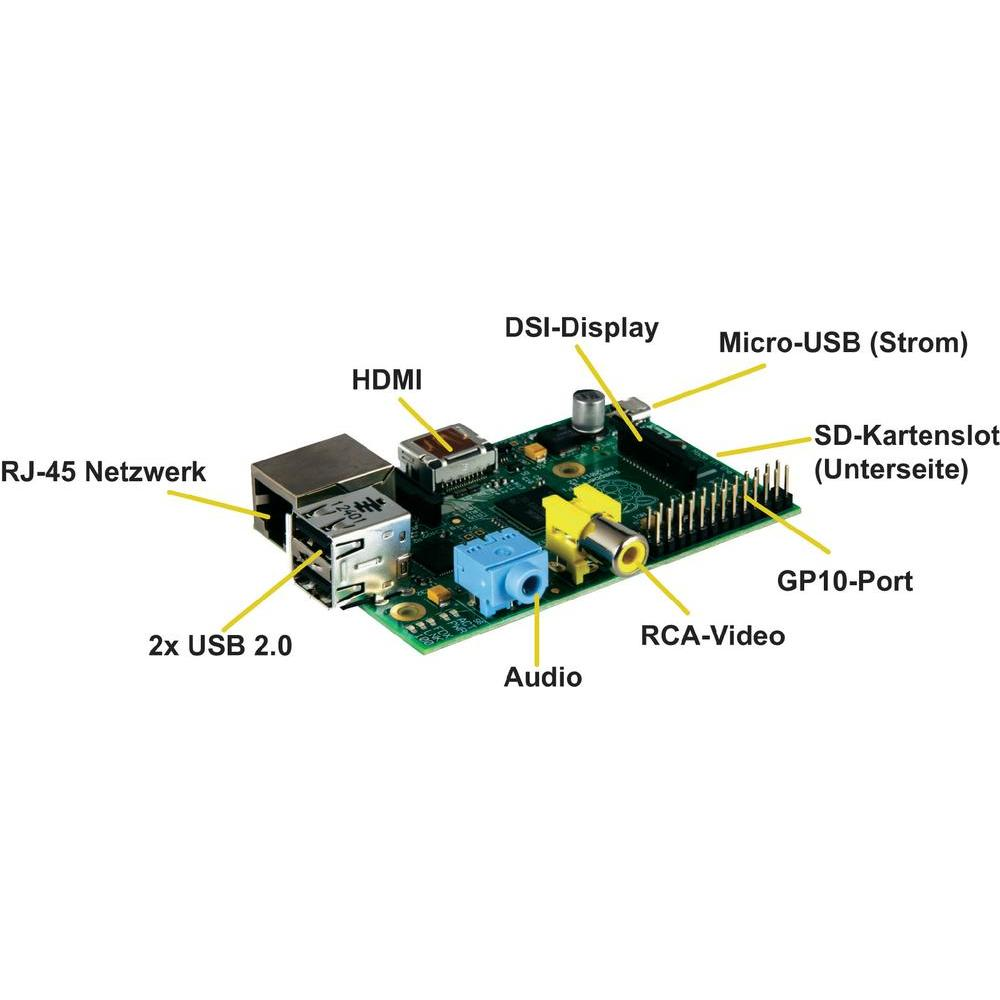
\includegraphics[width=1\textwidth]{Images/RaspberryPi.jpg}
\caption{Pi (Quelle www.Conrad.ch)}
\label{fig:raspi}
\end{figure}

\subsubsection{GPIO}
General-purpose input/output (GPIO) ist ein digitaler Anschlusspunkt, welcher vom Raspberry Pi zur Verfügung gestellt wird. Über diese Schnittstelle können die Werte der angeschlossenen Sensoren übertragen werden. Für die Auswertung analoger Sensoren muss entsprechend ein Analog- Digitalwandler verwendet werden.\\
Digitale Sensoren wie z.B. ein LM75 können direkt angeschlossen und über $I^2C$ verwendet werden, sind in der Anschaffung dafür etwas teurer (mikrocontroller.net).

\subsubsection{Sensortypen}
Um eine Temperaturmessung zu realisieren stehen diverse Sensortypen zu Verfügung. Einige analoge Sensortypen, wie PTC\footnote{Kaltleiter} und NTC\footnote{Heissleiter} verändern dabei ihren Widerstand in Abhängigkeit zur Temperatur, jedoch verläuft die Kurve nicht linear. Weitere Sensortypen sind elektronische Bauteile, die ein vorverarbeitetes Signal liefern, entweder einen linear angepassten Strom oder eine Spannung. Um den Berechnungsaufwand möglichst klein zu halten, wurde der Fokus auf die letzteren Sensortypen gelegt.\\
Nachteil der analogen Sensoren ist, dass auf dem Raspberry Pi nur digitale Eingänge (GPIO) zur Verfügung stehen. Es muss somit  mit einem Analog- Digitalwandler gearbeitet werden.


\subsection{Software Entwurfsmuster}
Die Software für die Temperaturüberwachung muss aufgrund des Dauerbetriebes, robust, energieschonend und erweiterbar gestaltet werden. Um diese Anforderungen zu erreichen, haben wir einige Entwurfsmuster verwendet.\\
Der Zugriff auf die Sensorwerte soll mittels eines Singleton-Pattern realisiert werden, damit keine parallelen Zugriffe erfolgen, wenn auch keine notwendig sind. Ebenso soll dieses Pattern für die Ausgabe der Log-Meldungen zum Einsatz kommen.\\
Die Sensoren müssen nicht im Dauerlauf abgefragt werden, da sich die Temperatur selten im Sekundentakt ändert. Deshalb sollen die Sensoren alle fünf bis zehn Sekunden ihre Werte rapportieren und nicht gepollt werden. Diese Anforderung soll mit dem Observer-Pattern erreicht werden.\\
Um eine regelmässige Prüfung der Sensoren sicherzustellen, wird ein Watchdog erstellt, welcher regelmässig über alle Kanäle iteriert und aktive, sowie inaktive Sensoren meldet. Werden neue Sensoren registriert, soll für jeden Sensor ein Thread gestartet werden. Fällt ein Sensor aus, oder wird entfernt, so wird der entsprechende Thread gestoppt.\\
Für die Anzeige der Sensordaten in der Webansicht, werden die Sensordaten von einer XML-Datei verwendet, welche mittels Pugixml\footnote{Pugixml ist ein leichtgewichtiger, open Source XML-Parser. www.pugixml.org} gelesen und verändert werden kann. Die gleiche XML-Datei soll für alle benötigten Konfigurationen verwendet werden.\\
Basierend auf den Erfahrungen des Teams, soll die Software in C++ realisiert werden.
